% Options for packages loaded elsewhere
\PassOptionsToPackage{unicode}{hyperref}
\PassOptionsToPackage{hyphens}{url}
\documentclass[
  11pt,
]{article}
\usepackage{xcolor}
\usepackage[margin=1in,bottom=.82in]{geometry}
\usepackage{amsmath,amssymb}
\setcounter{secnumdepth}{-\maxdimen} % remove section numbering
\usepackage{iftex}
\ifPDFTeX
  \usepackage[T1]{fontenc}
  \usepackage[utf8]{inputenc}
  \usepackage{textcomp} % provide euro and other symbols
\else % if luatex or xetex
  \usepackage{unicode-math} % this also loads fontspec
  \defaultfontfeatures{Scale=MatchLowercase}
  \defaultfontfeatures[\rmfamily]{Ligatures=TeX,Scale=1}
\fi
\usepackage{lmodern}
\ifPDFTeX\else
  % xetex/luatex font selection
\fi
% Use upquote if available, for straight quotes in verbatim environments
\IfFileExists{upquote.sty}{\usepackage{upquote}}{}
\IfFileExists{microtype.sty}{% use microtype if available
  \usepackage[]{microtype}
  \UseMicrotypeSet[protrusion]{basicmath} % disable protrusion for tt fonts
}{}
\makeatletter
\@ifundefined{KOMAClassName}{% if non-KOMA class
  \IfFileExists{parskip.sty}{%
    \usepackage{parskip}
  }{% else
    \setlength{\parindent}{0pt}
    \setlength{\parskip}{6pt plus 2pt minus 1pt}}
}{% if KOMA class
  \KOMAoptions{parskip=half}}
\makeatother
\usepackage{longtable,booktabs,array}
\newcounter{none} % for unnumbered tables
\usepackage{calc} % for calculating minipage widths
% Correct order of tables after \paragraph or \subparagraph
\usepackage{etoolbox}
\makeatletter
\patchcmd\longtable{\par}{\if@noskipsec\mbox{}\fi\par}{}{}
\makeatother
% Allow footnotes in longtable head/foot
\IfFileExists{footnotehyper.sty}{\usepackage{footnotehyper}}{\usepackage{footnote}}
\makesavenoteenv{longtable}
\usepackage{graphicx}
\makeatletter
\newsavebox\pandoc@box
\newcommand*\pandocbounded[1]{% scales image to fit in text height/width
  \sbox\pandoc@box{#1}%
  \Gscale@div\@tempa{\textheight}{\dimexpr\ht\pandoc@box+\dp\pandoc@box\relax}%
  \Gscale@div\@tempb{\linewidth}{\wd\pandoc@box}%
  \ifdim\@tempb\p@<\@tempa\p@\let\@tempa\@tempb\fi% select the smaller of both
  \ifdim\@tempa\p@<\p@\scalebox{\@tempa}{\usebox\pandoc@box}%
  \else\usebox{\pandoc@box}%
  \fi%
}
% Set default figure placement to htbp
\def\fps@figure{htbp}
\makeatother
% definitions for citeproc citations
\NewDocumentCommand\citeproctext{}{}
\NewDocumentCommand\citeproc{mm}{%
  \begingroup\def\citeproctext{#2}\cite{#1}\endgroup}
\makeatletter
 % allow citations to break across lines
 \let\@cite@ofmt\@firstofone
 % avoid brackets around text for \cite:
 \def\@biblabel#1{}
 \def\@cite#1#2{{#1\if@tempswa , #2\fi}}
\makeatother
\newlength{\cslhangindent}
\setlength{\cslhangindent}{1.5em}
\newlength{\csllabelwidth}
\setlength{\csllabelwidth}{3em}
\newenvironment{CSLReferences}[2] % #1 hanging-indent, #2 entry-spacing
 {\begin{list}{}{%
  \setlength{\itemindent}{0pt}
  \setlength{\leftmargin}{0pt}
  \setlength{\parsep}{0pt}
  % turn on hanging indent if param 1 is 1
  \ifodd #1
   \setlength{\leftmargin}{\cslhangindent}
   \setlength{\itemindent}{-1\cslhangindent}
  \fi
  % set entry spacing
  \setlength{\itemsep}{#2\baselineskip}}}
 {\end{list}}
\usepackage{calc}
\newcommand{\CSLBlock}[1]{\hfill\break\parbox[t]{\linewidth}{\strut\ignorespaces#1\strut}}
\newcommand{\CSLLeftMargin}[1]{\parbox[t]{\csllabelwidth}{\strut#1\strut}}
\newcommand{\CSLRightInline}[1]{\parbox[t]{\linewidth - \csllabelwidth}{\strut#1\strut}}
\newcommand{\CSLIndent}[1]{\hspace{\cslhangindent}#1}
\setlength{\emergencystretch}{3em} % prevent overfull lines
\providecommand{\tightlist}{%
  \setlength{\itemsep}{0pt}\setlength{\parskip}{0pt}}
\usepackage{bookmark}
\IfFileExists{xurl.sty}{\usepackage{xurl}}{} % add URL line breaks if available
\urlstyle{same}
\hypersetup{
  pdftitle={When Should an Assistant Check a Memory Update?},
  hidelinks,
  pdfcreator={LaTeX via pandoc}}

\title{When Should an Assistant Check a Memory Update?}
\usepackage{etoolbox}
\makeatletter
\providecommand{\subtitle}[1]{% add subtitle to \maketitle
  \apptocmd{\@title}{\par {\large #1 \par}}{}{}
}
\makeatother
\subtitle{A budget-matched replay study of temporal memory}
\author{}
\date{}

\begin{document}
\maketitle

\section{Abstract}\label{abstract}

A memory assistant can spend an extra model call to check whether a new
statement supersedes a stored fact. Checking one update changes which
fact the next statement can contradict. We study how this dependence
affects the evaluation of verification policies. Across 100 fictional
histories, a learned allocation policy and a paced heuristic each spent
250 verifier calls. When each policy acted on its own evolving memory,
the learned policy passed 434 of 600 exact state checks and the
heuristic passed 394, a difference of +6.7 percentage points (paired
family-bootstrap 95\% interval +0.7 to +12.3). When selecting from a
common stream of candidate conflicts, the same policies passed 341 and
409 checks, respectively, reversing their ranking. A chronological
baseline that checked the earliest conflicts reached 68.7\%, and the
paired interval for the learned policy's advantage over this baseline
included zero. Overestimating future opportunities further favored the
early-call baseline. Reader and external diagnostics showed substantial
losses between correct state and correct answers. These findings support
evaluating verification policies on their own trajectories and reporting
realized expenditure alongside memory quality.

\section{Introduction}\label{introduction}

Suppose a user moves from Halifax to Ottawa, then mentions a week in
Montréal. The assistant must decide which statements describe residence,
which date each describes, and whether it may retain the information. An
error at the first move changes the comparison at the next turn. A
verifier asked about Montréal versus Halifax faces a different question
from one asked about Montréal versus Ottawa. With only one extra call
available, the assistant also has to decide whether to spend it now.

This paper asks whether a learned controller makes better use of a
scarce verifier than a simple allocation rule. We examine two
experimental designs. In one, every policy sees the conflicts identified
by a common reference store. In the other, each policy discovers
conflicts in the state it has actually produced. The first design
controls candidate availability. The second measures the consequences of
deploying the policy over a sequence. A ranking that transfers between
them would simplify offline evaluation.

The same frozen scores yield opposite rankings under these two designs
at identical expenditure. This counterexample matters for developers
using a cheap, common candidate pool to select a policy that will
control a changing store. We then test how the conclusion changes with a
simpler baseline and a misspecified horizon. Finally, we follow the
evidence downstream to distinguish a correct memory state from a correct
user-facing answer. The latter distinction matters for assistants whose
reader can abstain, select the wrong date, or fail to receive a fact in
the first place.

\section{Related work}\label{related-work}

Temporal memory systems differ in the decision they evaluate. Zep
retains temporal graph relationships, while A-MEM organizes notes and
evolves their links (\citeproc{ref-rasmussen2025zep}{Rasmussen et al.
2025}; \citeproc{ref-xu2025amem}{Xu et al. 2025}). Mem0 extracts and
consolidates salient conversation content
(\citeproc{ref-chhikara2025mem0}{Chhikara et al. 2025}). MemFSM
distinguishes validity from visibility across a memory lifecycle, and
TOKI treats contradiction resolution as a bitemporal write with explicit
operators (\citeproc{ref-zhou2026validity}{Zhou et al. 2026};
\citeproc{ref-wang2026toki}{Wang 2026}). All provide reasons to model
supersession explicitly. Our comparison holds a transition system fixed
and varies which competing writes receive extra inference. It supplies
no head-to-head performance estimate against those architectures.

FlexA-Mem varies the detail of retrieved memory under a token budget
(\citeproc{ref-xu2026flexamem}{Xu et al. 2026}). FrugalGPT allocates
model expenditure across calls and Adaptive-Consistency varies the
number of samples as agreement emerges
(\citeproc{ref-chen2023frugalgpt}{Chen et al. 2023};
\citeproc{ref-aggarwal2023adaptive}{Aggarwal et al. 2023}).
Chain-of-Verification checks a drafted answer
(\citeproc{ref-dhuliawala2024cove}{Dhuliawala et al. 2024}). Here the
scarce unit is one logical check on a write. Spending that unit can
change the identity of a later candidate. Memora evaluates remembering
alongside forgetting, and LongMemEval distinguishes indexing, retrieval
and reading (\citeproc{ref-uddin2026memora}{Uddin et al. 2026};
\citeproc{ref-wu2025longmemeval}{Wu et al. 2025}). We use the two
external diagnostics to test the limits of conclusions drawn from
exact-state accuracy.

\section{Temporal state and
verification}\label{temporal-state-and-verification}

TRACE-Mem associates a claim with an entity, predicate, value, source,
and temporal bounds. Observation order determines when the system sees a
statement. Effective time determines which value it should return for a
particular date. A replacement may end the prior value's current
validity while leaving it available for an authorized historical
question. A deletion can also remove its visibility for historical
questions. The reader receives only authorized facts projected from
retained state. Pending or rejected claims do not supply evidence.

The controlled experiment supplies candidate claims and tests conflicts
on an exact entity and predicate match. The base transition rule (B2)
processes a candidate without purchasing a verifier call. An allocation
policy can spend a call to adjudicate a conflict. B3 spends on the
earliest eligible conflicts until its allowance runs out. H-paced uses a
hand-designed score to pace expenditure against expected remaining
opportunities. T2 uses the same pacing mechanism with a frozen learned
score and natural language inference features. The comparison changes
both the score source and feature availability. T2's scoring model was
developed on a separate synthetic release of 200 histories in 40 family
groups. The labeled training, calibration, and evaluation portions
contained 112, 63, and 37 candidate outcomes. Weights remained frozen
for the experiments reported here.

In fixed-stream evaluation, each policy selects targets from the common
B2 conflict stream. If earlier decisions have superseded a selected
target, the call counts against the budget and the transition falls back
to B2. This prevents applying a verdict to the wrong fact. In
chronological evaluation, candidates are checked against the policy's
own live state at arrival. Each policy may therefore encounter a
different set of eligible targets or finish with unspent calls.

The learned score is a calibrated logistic estimate of verification
helpfulness. T1 thresholds it at the actual remaining-budget coordinate.
T2 fixes that coordinate to one and compares the score with the upper
tail of its training reference. The remaining calls divided by the
remaining planned opportunities sets the size of that tail. The
accompanying master manuscript gives the equations, pseudocode and
implementation mapping.

\section{Experimental design}\label{experimental-design}

The primary study used 100 generated histories in ten authored domain
families (data seed 61843). Each history contained two genuine
replacements, a misleading correction, an uncertain proposal, an
archival mention, a deletion, unrelated material, and two expenses.
Dates, evidence order, and values varied. Prepared candidates included a
false correction and a true correction expressed as an assertion.
Supplying candidates controls an upstream source of variation but leaves
autonomous extraction outside the primary experiment.

The reference stream contained five conflicts per history. The budget
grid allowed 0, 50, 125, 250, or 500 logical verifier calls across the
cohort. The prespecified primary comparison was T2 versus H-paced at 250
allowed calls, analyzed separately in each replay design. Both paced
policies initially expected five opportunities per history. A logical
call records one policy decision to use the verifier, including a call
whose result can be reused from cache. It measures expenditure in
decisions. Prompt length and fresh compute can still vary.

The primary outcome is exact slot accuracy over six checks per history:
the five dates immediately following candidate turns, evaluated
retrospectively, and the final state. Retaining the correct value
alongside an incorrect value fails an exact check. The timeline supplies
the expected values independently of the verifier. Each paired interval
resamples the ten family groups 2,000 times (seed 9001), retaining both
policies' outcomes within each draw. The intervals are unadjusted. They
describe variation across a small set of related authored families.

The follow-up changed the expected horizon to 2, 3, 5, 7, or 10 while
holding the allowance fixed. Its protocol was frozen before the
follow-up runs, after the primary cohort had been examined. We treat
these results as robustness checks. A separate reader analysis sampled
three histories per family and counted invalid, contradictory, and
abstained short answers in the denominator.

\section{Results}\label{results}

\textbf{Table 1. Exact temporal-state accuracy at the nominal 50\%
allowance.} Each cell summarizes 600 checks. Parentheses give logical
verifier calls. The primary pair spent the full allowance in both
designs.

{\def\LTcaptype{none} % do not increment counter
\begin{longtable}[]{@{}lrr@{}}
\toprule\noalign{}
Policy & Common conflict stream & Own chronological state \\
\midrule\noalign{}
\endhead
\bottomrule\noalign{}
\endlastfoot
Base transitions (B2) & 37.0\% (0) & 37.0\% (0) \\
Earliest calls (B3) & 59.3\% (250) & 68.7\% (250) \\
Paced heuristic & 68.2\% (250) & 65.7\% (250) \\
Paced learned policy & 56.8\% (250) & 72.3\% (250) \\
\end{longtable}
}

\textbf{Replay design changes the ranking.} On the common stream T2
passed 341 checks and H-paced passed 409, a difference of −11.3
percentage points (95\% interval −16.3 to −6.3). On their own
trajectories the totals were 434 and 394, a difference of +6.7 points
(+0.7 to +12.3). In fixed replay, 94 selected T2 targets and 70
heuristic targets had become stale. In chronological replay, 122 applied
T2 verifications improved the immediate disposition relative to B2,
versus 85 for H-paced. These diagnostics are consistent with
consequential differences in target selection. Staleness, timing, and
state changed together, so their individual causal contributions remain
unresolved.

\begin{figure}
\centering
\pandocbounded{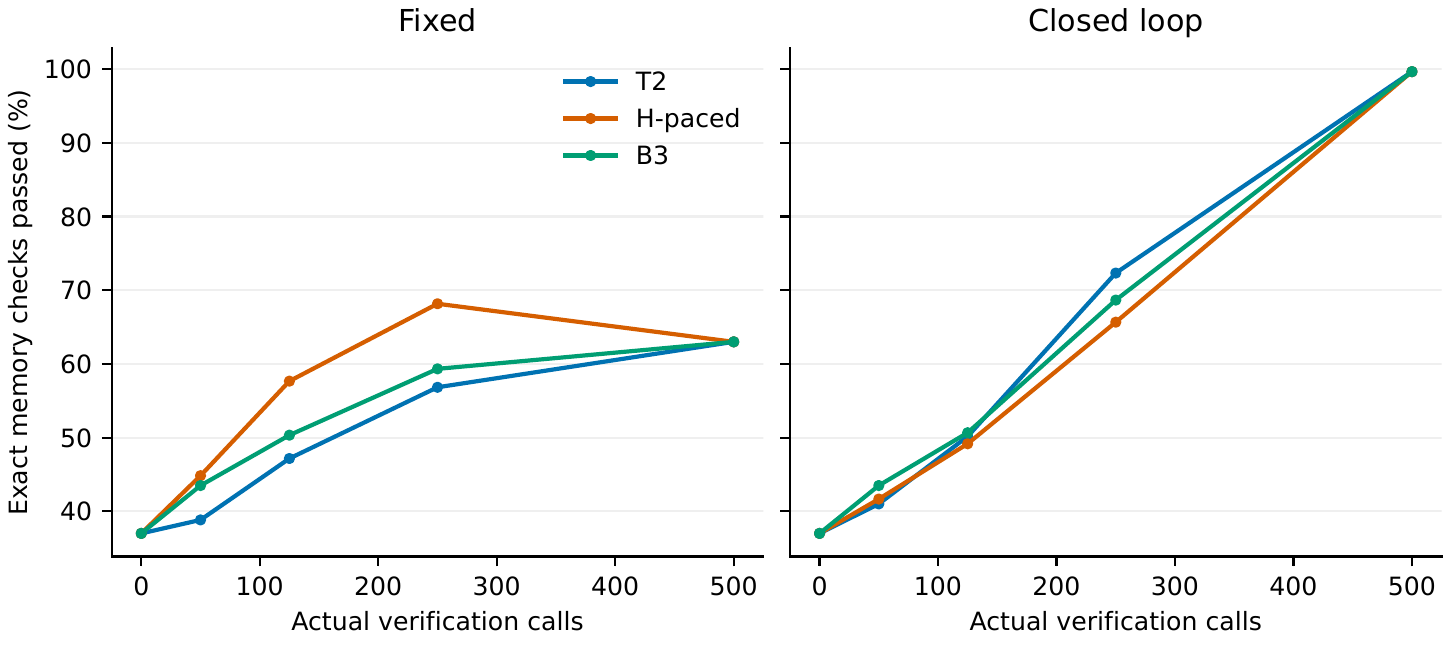
\includegraphics[keepaspectratio,alt={Exact temporal-state accuracy versus realized verifier calls. The nominal 50\% comparison pairs the same histories and 250 calls in both replay designs. Lines join evaluated budget settings.}]{budget-reversal.png}}
\caption{Exact temporal-state accuracy versus realized verifier calls.
The nominal 50\% comparison pairs the same histories and 250 calls in
both replay designs. Lines join evaluated budget settings.}
\end{figure}

\textbf{A simpler competitor narrows the result.} T2 exceeded early-call
B3 by 3.7 points at the nominal chronological horizon (95\% interval
−1.7 to +9.0). B3 led at both the 10\% and 25\% allowances with equal
spending. With 500 calls, B3, H-paced, and T2 each passed 598/600
chronological checks. An oracle applying the authored update decisions
passed all 600. At twice the nominal horizon, T2 saved calls for
opportunities that never arrived. It spent 211/250 calls and scored
59.0\%, while B3 spent 250 and scored 68.7\% (difference −9.7 points,
interval −16.3 to −3.2). This comparison measures the practical effect
of the planning assumption, including its effect on spending.

\textbf{State accuracy does not predict reader accuracy on this sample.}
On 30 chronological short-answer questions at the nominal horizon, T2
answered 7 correctly, B3 answered 6, and H-paced answered 12. In the
earlier ten-history subset even the oracle state yielded only five
correct generated short answers, while its deterministic expense
subtotal was correct on all ten. Reader failures can therefore persist
after update decisions have been resolved. The samples are too small for
a stable ranking of readers.

\textbf{Resource use.} The primary grid completed in 1,021 seconds on an
RTX 2060 system. Across conditions and seeds, 16,489 logical verifier
calls required 814 fresh requests after cache reuse. Fresh verification
consumed 233,459 input tokens, 9,537 output tokens, and 730.4 seconds of
summed request latency. Shared caching reduces the cost of running the
grid. These totals cannot be interpreted as the serving latency of one
policy.

\section{From memory state to user-facing
answers}\label{from-memory-state-to-user-facing-answers}

The external diagnostics expose substantial attrition. The Memora
development run scored zero adapted FAMA across scored conditions. On
LongMemEval, BM25, MiniLM and oracle evidence yielded 3/14, 2/14 and
6/14 correct. Managed replay completed one case and missed it. The
candidate extractor recovered 50/100 facts and the revised reader
declined from 27/30 to 24/30. Both missed promotion gates.

A separate Workspace engineering pilot used reviewed facts and one
trajectory with six nested prefixes, approximately 1k--64k accumulated
tokens. The three probes at each prefix share evidence. Recent history,
hybrid retrieval and TRACE-Mem answered 0/18, 6/18 and 18/18 correctly.
Both retrieval modes solved all six generated calculations. The
difference came from twelve deterministic temporal lookups. No verifier
ran; the native context size stayed fixed. MiniLM found one of four
paraphrases at rank one and lexical retrieval found none.

\section{Limitations and
implications}\label{limitations-and-implications}

The strongest claim concerns the evaluation design. Freezing candidates
makes two selectors comparable at the point of ranking. It can also
reward a different selector from the one whose decisions maintain a more
accurate live state. Reporting both designs exposes that discrepancy.
Reporting an early-call baseline further reveals whether a learned
policy improves on simply spending while opportunities are present.

Several boundaries constrain interpretation. The study controls claim
availability and reuses update archetypes across ten families. Family
resampling captures only part of that dependence. Horizon perturbations
reuse the original histories. Scores and language-inference features
differ together. Call matching does not equalize tokens or energy. The
Workspace experiment begins with reviewed evidence, and its nested
histories share a single source turn. An independent evaluation would
need fresh scenario authors or independently sourced histories, a
prespecified comparison with early-call and paced allocation, realistic
extraction, and enough completed external trajectories for paired answer
scoring. Our current data cannot resolve whether the learned policy
improves a deployed assistant.

\section{Ethics, artifacts, and
reproducibility}\label{ethics-artifacts-and-reproducibility}

The primary histories and Workspace trajectory are fictional.
Authorization is applied when facts are projected to the reader,
including at historical dates. All 28,000 repeated synthetic
policy-level privacy checks passed across the primary grid. Repeated
checks share scenarios and do not demonstrate comprehensive privacy or
resistance to adversarial input. Human-assisted annotations in earlier
project development were kept separate from the primary experiment. No
participant outcomes are reported here.

The primary protocol and dataset hash were frozen at commit 486e576, the
horizon follow-up at b6aa346, and the Workspace fixtures at 6fe317d with
measured candidate f93c13b. Raw third-party benchmark answers, private
annotations, and model checkpoints are excluded from the numeric
release. The public artifact (\citeproc{ref-tracemem}{TRACE-Mem project
2026}) includes sanitized outcome counts, family identifiers, a
manifest, and a standard-library reproduction script. From the
reproducibility directory, running ``python reproduce.py --output
reproduced'' recomputes 230 condition summaries and 184 intervals. This
checks arithmetic from archived observations. Repeating model inference
additionally requires the model versions and local dependencies in the
run manifests. AI assistance was used in project development and in
drafting this manuscript. The internally authored fixtures and automated
analyses have not undergone independent scientific replication.

\section{Conclusion}\label{conclusion}

At the same 250-call expenditure, replaying a common set of conflicts
and maintaining a live temporal store produced opposite rankings of two
verification policies. An early-call policy remained competitive, and a
longer assumed horizon left useful calls unspent. For conversational
memory research, the outcome worth measuring is the sequence from
candidate acquisition through state changes to authorized answers. In
this study, a gain at one stage was insufficient to establish a gain at
the next.

References

\protect\phantomsection\label{refs}
\begin{CSLReferences}{1}{1}
\bibitem[\citeproctext]{ref-aggarwal2023adaptive}
Aggarwal, Pranjal, Aman Madaan, Yiming Yang, and Mausam. 2023.
\emph{Let's Sample Step by Step: Adaptive-Consistency for Efficient
Reasoning and Coding with LLMs}. \url{https://arxiv.org/abs/2305.11860}.

\bibitem[\citeproctext]{ref-chen2023frugalgpt}
Chen, Lingjiao, Matei Zaharia, and James Zou. 2023. \emph{{FrugalGPT}:
How to Use Large Language Models While Reducing Cost and Improving
Performance}. \url{https://arxiv.org/abs/2305.05176}.

\bibitem[\citeproctext]{ref-chhikara2025mem0}
Chhikara, Prateek, Dev Khant, Saket Aryan, Taranjeet Singh, and Deshraj
Yadav. 2025. \emph{{Mem0}: Building Production-Ready AI Agents with
Scalable Long-Term Memory}. \url{https://arxiv.org/abs/2504.19413}.

\bibitem[\citeproctext]{ref-dhuliawala2024cove}
Dhuliawala, Shehzaad, Mojtaba Komeili, Jing Xu, et al. 2024.
{``Chain-of-Verification Reduces Hallucination in Large Language
Models.''} \emph{Findings of the Association for Computational
Linguistics: ACL 2024}, 3563--78.
\url{https://doi.org/10.18653/v1/2024.findings-acl.212}.

\bibitem[\citeproctext]{ref-rasmussen2025zep}
Rasmussen, Preston, Pavlo Paliychuk, Travis Beauvais, Jack Ryan, and
Daniel Chalef. 2025. \emph{Zep: A Temporal Knowledge Graph Architecture
for Agent Memory}. \url{https://arxiv.org/abs/2501.13956}.

\bibitem[\citeproctext]{ref-tracemem}
TRACE-Mem project. 2026. \emph{Offline Evidence Package, Experimental
Protocols, and Workspace Pilot Observations}.
\url{https://github.com/Harmit3/TRACE-Mem/tree/da4c491}.

\bibitem[\citeproctext]{ref-uddin2026memora}
Uddin, Md Nayem, Kumar Shubham, Eduardo Blanco, Chitta Baral, and Gengyu
Wang. 2026. {``From Recall to Forgetting: Benchmarking Long-Term Memory
for Personalized Agents.''} \emph{Findings of the Association for
Computational Linguistics: ACL 2026}, 26814--41.
\url{https://doi.org/10.18653/v1/2026.findings-acl.1337}.

\bibitem[\citeproctext]{ref-wang2026toki}
Wang, Ziming. 2026. \emph{{TOKI}: A Bitemporal Operator Algebra for
Contradiction Resolution in LLM-Agent Persistent Memory}.
\url{https://arxiv.org/abs/2606.06240}.

\bibitem[\citeproctext]{ref-wu2025longmemeval}
Wu, Di, Hongwei Wang, Wenhao Yu, Yuwei Zhang, Kai-Wei Chang, and Dong
Yu. 2025. {``{LongMemEval}: Benchmarking Chat Assistants on Long-Term
Interactive Memory.''} \emph{International Conference on Learning
Representations}. \url{https://arxiv.org/abs/2410.10813}.

\bibitem[\citeproctext]{ref-xu2026flexamem}
Xu, Wujiang, Jiaojiao Han, Xi Zhu, et al. 2026. \emph{{FlexA-Mem}:
Budget-Adaptive Agentic Memory for LLM Agents}.
\url{https://arxiv.org/abs/2610.33274}.

\bibitem[\citeproctext]{ref-xu2025amem}
Xu, Wujiang, Zujie Liang, Kai Mei, Hang Gao, Juntao Tan, and Yongfeng
Zhang. 2025. {``{A-MEM}: Agentic Memory for LLM Agents.''}
\emph{Advances in Neural Information Processing Systems} 38.
\url{https://arxiv.org/abs/2502.12110}.

\bibitem[\citeproctext]{ref-zhou2026validity}
Zhou, Shuo, Pengcheng Xu, Shaotong Qi, Li Que, Ming Sun, and Han Li.
2026. {``Validity Is Not Visibility: A Lifecycle FSM for Agent
Memory.''} \emph{Proceedings of the 2026 Conference on Empirical Methods
in Natural Language Processing}, 5895--913.
\url{https://doi.org/10.18653/2026.emnlp-main.260}.

\end{CSLReferences}

\end{document}
